\documentclass[12pt,fleqn]{article}\usepackage{../common}
\begin{document}
Ortalama Kaydirma ile Kumeleme (Mean Shift Clustering)

Kumeleme yapmak icin bir metot daha: Ortalama Kaydirma metotu. Bu
metodun mesela K-Means'den farki kume sayisinin onceden belirtilmeye
ihtiyaci olmamasidir, kume sayisi otomatik olarak metot tarafindan
saptanir.

"Kume" olarak saptanan aslinda veri icindeki tum yogunluk bolgelerinin
merkezleridir, yani alttaki resmin sag kismindaki bolgeler. 

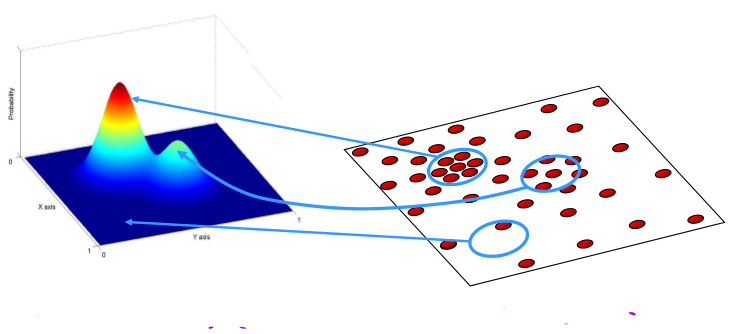
\includegraphics[height=6cm]{dist.png}

Baslangic neresidir? Baslangic tum noktalardir, yani her noktadan
baslanarak

1. O nokta etrafinda (yeterince buyuk) bir pencere tanimla

2. Bu pencere icine dusen tum noktalari hesaba katarak bir ortalama yer hesapla

3. Pencereyi yeni ortalama noktayi merkezine alacak sekilde kaydir

Metotun ismi buradan geliyor, cunku pencere yeni ortalamaya dogru
"kaydiriliyor". Altta bir noktadan baslanarak yapilan hareketi
goruyoruz.  Kaymanin saga dogru olmasi mantikli cunku tek pencere
icinden bakinca bile yogunlugun "sag tarafa dogru" oldugu
gorulmekte. Yontemin puf noktasi burada.

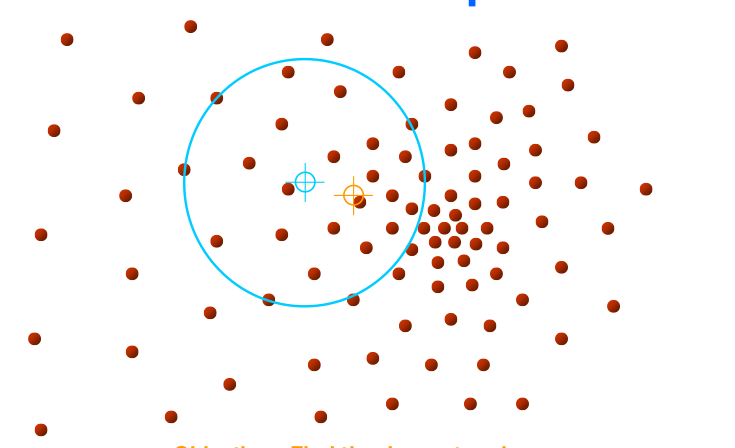
\includegraphics[height=6cm]{mean_2.png}

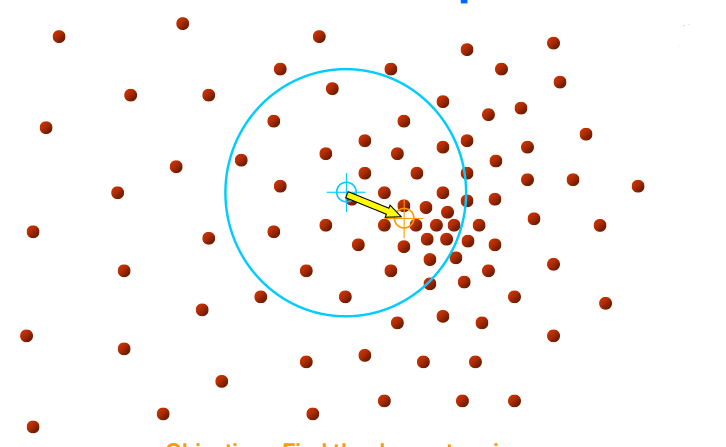
\includegraphics[height=6cm]{mean_3.png}

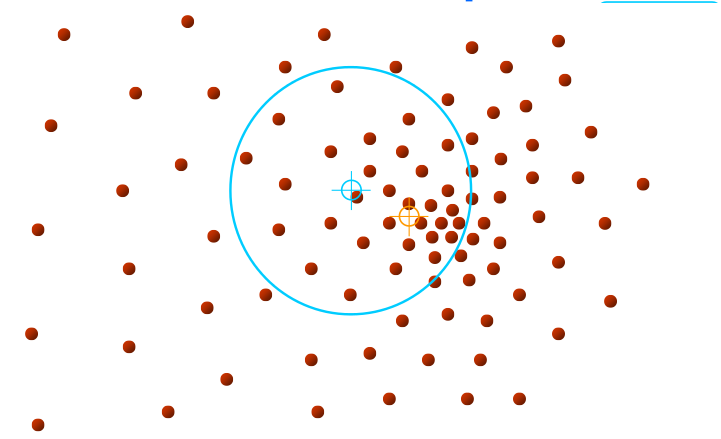
\includegraphics[height=6cm]{mean_4.png}

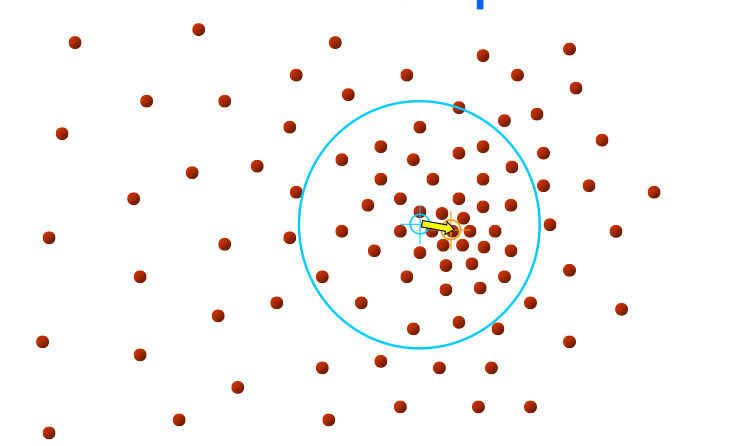
\includegraphics[height=6cm]{mean_5.png}

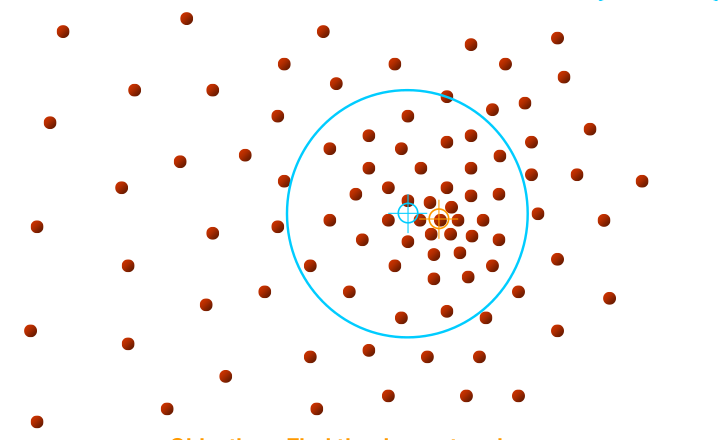
\includegraphics[height=6cm]{mean_6.png}

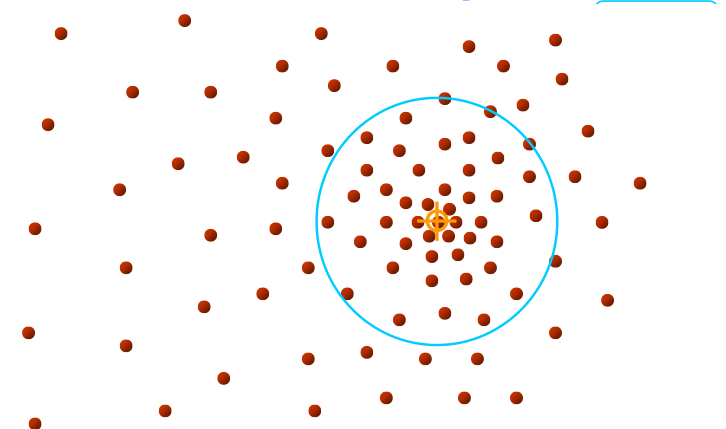
\includegraphics[height=6cm]{mean_7.png}

Eger yogunluk merkezine cok yakin bir noktadan / noktalardan
baslamissak ne olur?

O zaman ilerleme o baslangic noktasi icin aninda bitecek, cunku hemen
yogunluk merkezine gelmis olacagiz. Diger yonlerden gelen pencereler
de ayni yere gelecekler tabii, o zaman ayni / yakin yogunluk
merkezlerini ayni kume olarak kabul etmemiz gerekir. Bu "ayni kume
irdelemesi" sayisal hesaplama acisindan ufak farklar gosterebilir
tabii, ve bu ufak farki gozonune alarak "kume birlestirme" mantigini da
eklemek gerekiyor.

Ortalama Kaydirma sisteminde pencere buyuklugu kullanici tarafindan
tanimlanir.  Optimal pencere buyuklugunu nasil buluruz? Deneme yanilma
yontemi, verinin tarifsel istatistiklerine kestirme bir hesap
(estimate) etmek, ya da kullanicinin ayni istatistiklere bakarak
tahminde bulunmasi. Birkac farkli pencere buyuklugu de denenebilir. Bu
konu literaturde (Ing. bandwidth selection) adi atlinda uzun uzadiya
tartisilmaktadir. Fakat evet, kullanici tarafindan tanimli bu
parametrenin bir anlamda bu metotun bir zayifligi oldugu soylenebilir. KMeans
kume sayisini istiyordu, bu metot ta pencere buyuklugunu istiyor. Hangi
metotun ne zaman uygun oldugunu anlamak tecrube gerektiriyor. 

Eger yogunluk merkezine cok yakin bir noktadan / noktalardan
baslamissak ne olur?

O zaman ilerleme o baslangic noktasi icin aninda bitecek, cunku hemen
yogunluk merkezine gelmis olacagiz. Diger yonlerden gelen pencereler
de ayni yere gelecekler tabii, o zaman ayni / yakin yogunluk
merkezlerini ayni kume olarak kabul etmemiz gerekir. Bu "ayni kume
irdelemesi" sayisal hesaplama acisindan ufak farklar gosterebilir
tabii, ve bu ufak farki gozonune alarak "kume birlestirme" mantigini da
eklemek gerekiyor.

Ortalama Kaydirma sisteminde pencere buyuklugu kullanici tarafindan
tanimlanir.  Optimal pencere buyuklugunu nasil buluruz? Deneme yanilma
yontemi, verinin tarifsel istatistiklerine kestirme bir hesap
(estimate) etmek, ya da kullanicinin ayni istatistiklere bakarak
tahminde bulunmasi. Birkac farkli pencere buyuklugu de denenebilir. Bu
konu literaturde (Ing. bandwidth selection) adi atlinda uzun uzadiya
tartisilmaktadir. Fakat evet, kullanici tarafindan tanimli bu
parametrenin bir anlamda bu metotun bir zayifligi oldugu soylenebilir. KMeans
kume sayisini istiyordu, bu metot ta pencere buyuklugunu istiyor. Hangi
metotun ne zaman uygun oldugunu anlamak tecrube gerektiriyor. 

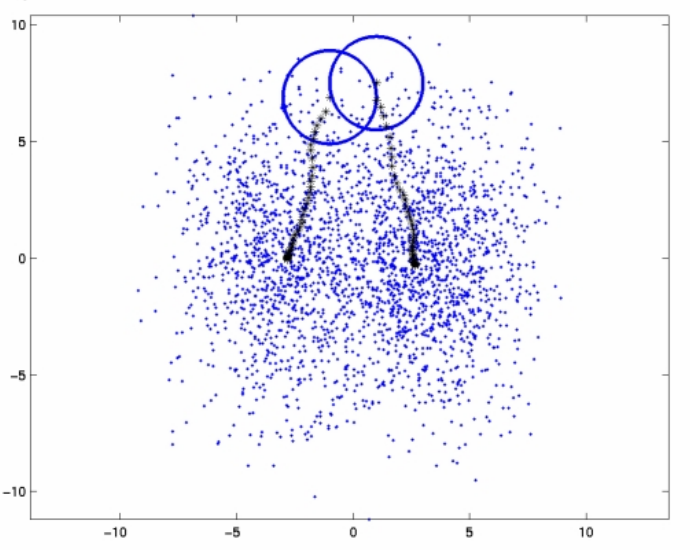
\includegraphics[height=6cm]{start.png}

Altta ornek veri ve kodu bulabilirsiniz (kod \verb!scikit-learn!
adli kutuphaneden alinmistir). Metot kume sayisi 17'yi otomatik olarak
buluyor.

Alternatif bir kod \verb!meanshift_alternative.py! dosyasinda
bulunabilir, bu kod pencereler kaydirirken onlarin uzerinden gectigi
noktalari "sahiplenen" turden bir kod. Yani [encere hareketini
durdurdugunda hem kume merkezini hem de o kumenin altindaki noktalari
bulmus oluyoruz.  Tabii sonraki pencereler bazi noktalari onceki
kumelerden calabilirler. Neyse, islemin normal isleyisine gore bir
sonraki pencere secilecektir ve bu pencere "geriye kalan noktalar"
uzerinden islem yapacaktir.  Beklenir ki, islem ilerledikce islenmesi
gereken noktalar azalacaktir ve yontemin bu sebeple klasik yonteme
gore daha hizli isleyecegi tahmin edilebilir. Hakikaten de boyledir.

\begin{minted}{python}
from pandas import *
data = read_csv("synthetic.txt",header=None,sep="   ")
print data.shape
data = np.array(data)
\end{minted}

\begin{verbatim}
(3000, 2)
\end{verbatim}

\begin{minted}{python}
%pylab inline
plt.scatter(data[:,0],data[:,1])
plt.savefig('meanshift_1.png')
\end{minted}

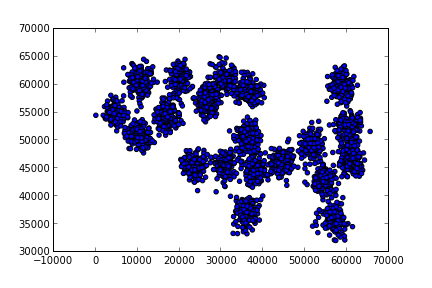
\includegraphics[height=6cm]{meanshift_1.png}
\begin{minted}{python}
import numpy as np
from sklearn.neighbors import NearestNeighbors
from sklearn.utils import extmath

def mean_shift(X, bandwidth=None, max_iterations=300):
    
    seeds = X
    n_samples, n_features = X.shape
    stop_thresh = 1e-3 * bandwidth  # when mean has converged
    center_intensity_dict = {}
    nbrs = NearestNeighbors(radius=bandwidth).fit(X)

    # For each seed, climb gradient until convergence or max_iterations
    for my_mean in seeds:
        completed_iterations = 0
        while True:
            # Find mean of points within bandwidth
            i_nbrs = nbrs.radius_neighbors([my_mean], bandwidth,
                                           return_distance=False)[0]
            points_within = X[i_nbrs]
            if len(points_within) == 0:
                break  # Depending on seeding strategy this condition may occur
            my_old_mean = my_mean  # save the old mean
            my_mean = np.mean(points_within, axis=0)
            # If converged or at max_iterations, addS the cluster
            if (extmath.norm(my_mean - my_old_mean) < stop_thresh or
                    completed_iterations == max_iterations):
                center_intensity_dict[tuple(my_mean)] = len(points_within)
                break
            completed_iterations += 1

    # POST PROCESSING: remove near duplicate points
    # If the distance between two kernels is less than the bandwidth,
    # then we have to remove one because it is a duplicate. Remove the
    # one with fewer points.
    sorted_by_intensity = sorted(center_intensity_dict.items(),
                                 key=lambda tup: tup[1], reverse=True)
    sorted_centers = np.array([tup[0] for tup in sorted_by_intensity])
    unique = np.ones(len(sorted_centers), dtype=np.bool)
    nbrs = NearestNeighbors(radius=bandwidth).fit(sorted_centers)
    for i, center in enumerate(sorted_centers):
        if unique[i]:
            neighbor_idxs = nbrs.radius_neighbors([center],
                                                  return_distance=False)[0]
            unique[neighbor_idxs] = 0
            unique[i] = 1  # leave the current point as unique
    cluster_centers = sorted_centers[unique]

    # ASSIGN LABELS: a point belongs to the cluster that it is closest to
    nbrs = NearestNeighbors(n_neighbors=1).fit(cluster_centers)
    labels = np.zeros(n_samples, dtype=np.int)
    distances, idxs = nbrs.kneighbors(X)
    labels = idxs.flatten()
    
    return cluster_centers, labels

cluster_centers, labels = mean_shift(np.array(data), 4000)

print len(cluster_centers)
\end{minted}

\begin{verbatim}
17
\end{verbatim}

\begin{minted}{python}
plt.scatter(data[:,0],data[:,1])
plt.hold(True)
for x in asarray(cluster_centers): plt.plot(x[0],x[1],'rd')
plt.savefig('meanshift_2.png')
\end{minted}

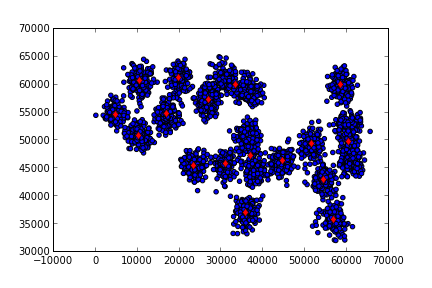
\includegraphics[height=6cm]{meanshift_2.png}
Teorik Konular

Bu metotu teorik bir yapiya oturtmak icin onu yazinin ilk basindaki
resimde oldugu gibi gormek gerekiyor, yani mesela o ilk resmin
sagindaki 2 boyuttaki veri dagilimi (ki ayriksal, sayisal), 3
boyuttaki surekli (continuous) bir baska dagilimin yansimasi sanki, ki
o zaman 2 boyuttaki yogunluk bolgeleri surekli dagilimdaki tepe
noktalarini temsil ediyorlar, ve biz o surekli versiyondaki tepe
noktalarini bulmaliyiz. Fakat kumeleme isleminin elinde sadece 2
boyuttaki veriler var, o zaman surekli dagilimi bir sekilde yaratmak
lazim.

Bunu yapmak icin problem / veri once bir Cekirdek Yogunluk Kestirimi
(Kernel Density Estimation -KDE-) problemi gibi goruluyor, ki her
nokta uzerine bir cekirdek fonksiyonu koyularak ve onlarin toplamim
alinarak sayisal dagilim puruzsuz bir hale getiriliyor. Ortalama
Kaydirma icin gerekli kayma "yonu" ise iste bu yeni surekli
fonksiyonun gradyanidir deniyor (elimizde bir surekli fonksiyon oldugu
icin turev rahatlikla alabiliyoruz), ve gradyan yerel tepe noktasini
gosterdigi icin o yone yapilan hareket bizi yavas yavas tepeye
goturecektir. Bu hareketin yerel tepeleri bulacagi, ve tum yontemin
nihai olarak sonuca yaklasacagi (convergence) matematiksel olarak
ispat edilebilir.

KDE ile elde edilen teorik dagilim fonksiyonunun icbukey olup olmadigi
onemli degil (ki mesela lojistik regresyonda bu onemliydi), cunku
nihai tepe noktasini degil, birkac yerel tepe noktasindan birini
(hatta hepsini) bulmakla ilgileniyoruz. Gradyan bizi bu noktaya
tasiyacaktir.

Kaynaklar

\verb!http://www.serc.iisc.ernet.in/~venky/SE263/slides/Mean-Shift-Theory.pdf!

\verb!http://saravananthirumuruganathan.wordpress.com/2010/04/01/introduction-to-mean-shift-algorithm/!

\verb!http://www.cse.yorku.ca/~kosta/CompVis_Notes/mean_shift.pdf!

\verb!http://homepages.inf.ed.ac.uk/rbf/CVonline/LOCAL_COPIES/TUZEL1/MeanShift.pdf!

Scikit-Learn Kodlari

\verb!http://yotamgingold.com/code/MeanShiftCluster.py!


\end{document}
